\documentclass[a4paper]{article}

%use the english line for english reports
%usepackage[english]{babel}
\usepackage[portuguese]{babel}
\usepackage[utf8]{inputenc}
\usepackage{indentfirst}
\usepackage{graphicx}
\usepackage{verbatim}
\usepackage{url}


\begin{document}

\setlength{\textwidth}{16cm}
\setlength{\textheight}{22cm}

\title{\Huge\textbf{Aplicação em Prolog para um Jogo de Tabuleiro}\linebreak\textbf{Cequis - Sumo}\linebreak\linebreak
\Large\textbf{Relatório Final}\linebreak\linebreak

\includegraphics[height=6cm, width=7cm]{feup.pdf}\linebreak \linebreak
\Large{Mestrado Integrado em Engenharia Informática e Computação} \linebreak \linebreak
\Large{Programação em Lógica}\linebreak
}

\author{\textbf{Grupo 45:}\\ Duarte Duarte - ei11101 \\ Hugo Freixo - ei11086 \\\linebreak\linebreak \\
 \\ Faculdade de Engenharia da Universidade do Porto \\ Rua Roberto Frias, s\/n, 4200-465 Porto, Portugal \linebreak\linebreak\linebreak
\linebreak\linebreak\vspace{1cm}}
%\date{Junho de 2007}
\maketitle
\thispagestyle{empty}

%************************************************************************************************
%************************************************************************************************

\newpage

\section*{Resumo}
No trabalho realizado pelo grupo foram encontrados vários problemas no percurso do seu desenvolvimento.
Um dos problemas foi o facto de o tabuleiro do nosso jogo ser constituído por hexágonos e não quadrados como na generalidade dos casos. Este problema foi resolvido bastante cedo com a criação específica da nossa lista de listas.
Uma primeira linha com menos elementos resolve o problema do nosso tabuleiro, como neste exemplo: 
\begin{verbatim}
[[e,    e,    e,    e],
 [e, e, e, e, e, e, e],
 [e, e, e, e, e, e, e],
 [e, e, e, e, e, e, e],
 [e, e, e, e, e, e, e],
 [e, e, e, e, e, e, e],
 [e, e, e, e, e, e, e],
 [e, e, e, e, e, e, e]]
\end{verbatim}

Outro problema que ocorreu foi o fato do jogo proposto ser o Cequis e o grupo ter escolhido Cequis-Sumo. O grupo resolveu continuar a implementação do Cequis-Sumo pois alguns predicados já estavam implementados e refazê-los tiraria tempo ao grupo de maneira que a finalização do Cequis seria impossível.

\newpage

\tableofcontents

%************************************************************************************************
%************************************************************************************************

%*************************************************************************************************
%************************************************************************************************

\newpage

\section{Introdução}

\section{O Jogo Cequis - Sumo}
Cequis - Sumo é um jogo de tabuleiro disputado entre dois adversários, que
possuem três pedras cada. O seu objetivo é retirar a pedra objetivo (ou branca)
da mesa, empurrando-a para fora do tabuleiro, antes que o jogador adversário
o faça. O tabuleiro consiste num conjunto de hexágonos ligados entre si desta
forma:\linebreak

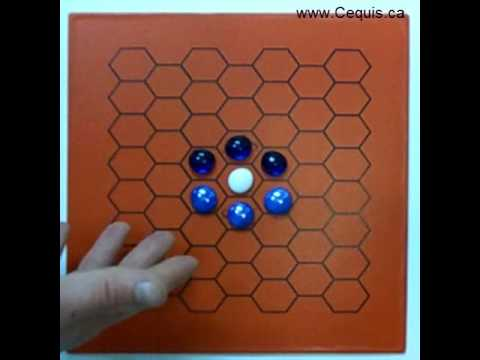
\includegraphics[height=6cm, width=7cm]{sumo.jpg}
\linebreak

Os jogadores podem andar para cima, baixo, cima-direita, cima-esquerda,
baixo-direita e baixo-esquerda e só podem efetuar um movimento por jogada.
O jogador pode mover uma pedra ou um conjunto de pedras. Um conjunto de
pedras são pedras da mesma cor que estão em espaços adjacentes.
É possivel empurrar pedras adversárias, sem as retirar do tabuleiro, mas
para isso é necessário um número igual ou superior de pedras que o número de
pedras que vamos empurrar. Podemos empurrar a pedra objetivo juntamente
com pedras adversárias, neste caso a pedra objetivo não tem "peso", ou seja
não é necessário uma pedra extra para a empurrar, apenas precisamos de cobrir
o número de pedras do nosso adversário que queremos empurrar.

\section{Arquitetura do Sistema}
O sistema está dividido em dois módulos: o módulo de Prolog, que trata de todo o processamento do jogo (desenrolar do jogo, verificação do cumprimento das regras do jogo, determinação do final do jogo) e o módulo de visualização, que ficará responsável por representar o jogo de uma forma intuitiva e apelativa, em 3D.

Para que este sistema funcione é necessário que os módulos comuniquem entre si, para isso existirá um sistema de comunicação entre os diferentes módulos. O sistema de comunicação será baseado em mensagens, por exemplo: move, init\_board, reset\_board, etc.

\section{Lógica do Jogo}

\subsection{Representação do Estado do Jogo}
O estado do tabuleiro será representado em Prolog recorrendo a uma lista de listas de peças válidas com a adição de uma peça fictícia para assinalar um espaço no tabuleiro sem peças.

\begin{itemize}
\item b - black - peça do jogador 1
\item w - white - peça do jogador 2
\item o - objective - peça objetivo
\item e - empty - posição sem peça
\end{itemize}

Estado inicial (tabuleiro de tamanho 8):
\begin{verbatim}
[[e,    e,    e,    e],
 [e, e, e, e, e, e, e],
 [e, e, e, e, e, e, e],
 [e, e, w, w, w, e, e],
 [e, e, b, o, b, e, e],
 [e, e, e, b, e, e, e],
 [e, e, e, e, e, e, e],
 [e, e, e, e, e, e, e]]
\end{verbatim}

Possível estado intermédio (tabuleiro de tamanho 8):
\begin{verbatim}
[[e,    e,    e,    e],
 [e, e, e, e, e, e, e],
 [e, e, e, e, e, e, o],
 [e, e, w, w, b, w, e],
 [e, e, b, e, b, b, e],
 [e, e, e, e, e, e, e],
 [e, e, e, e, e, e, e],
 [e, e, e, e, e, e, e]]
\end{verbatim}

Possível estado final (tabuleiro de tamanho 8):
\begin{verbatim}
[[e,    e,    e,    e],
 [e, e, e, e, e, e, e],
 [e, e, e, e, e, e, w],
 [e, e, e, w, b, w, e],
 [e, e, b, e, b, e, e],
 [e, e, e, e, e, e, e],
 [e, e, e, e, e, e, e],
 [e, e, e, e, e, e, e]]
\end{verbatim}

\subsection{Visualização do Estado do Jogo}
A visualização do tabuleiro em modo de texto é feita através da composição de caracteres ASCII. Para tal foi desenvolvido um conjunto de predicados, sendo show\_board/1 (que aceita uma lista de listas de peças por argumento) o predicado principal. Os predicados auxiliares são: draw\_piece/1, draw\_letters/1, draw\_letters\_aux/1, draw\_line\_numbers/1, draw\_slashes/1, draw\_lower\_cell/1, show\_line/2 e show\_piece/2.

O predicado show\_board/1 é génerico, ou seja, funciona com qualquer tamanho de tabuleiro (desde que a lista de listas de peças fornecidas seja válida).

O código destes predicados encontra-se em anexo.

Imagem do output produzido por show\_board/1:

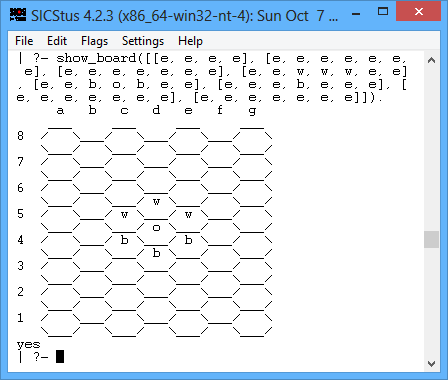
\includegraphics[height=6cm, width=7cm]{screenshot.png}

\subsection{Validação de Jogadas}
\textit{valid\_move(+Game, +Player, +LSrc, +CSrc, +LDest, +CDest, -LiSrc, -CiSrc, -LiDest, -CiDest)}

\begin{itemize}
\item \textit{+Game}: lista de listas de peças
\item \textit{+Player}: jogador que executou o movimento (\textit{player1, player2, computer1, computer2})
\item \textit{+LSrc,+CSrc}: posição da peça a mover (linha e coluna) escolhida pelo utilizador
\item \textit{+LDest,+CDest}: posição de destino da peça (linha e coluna) escolhida pelo utilizador
\item \textit{-LiSrc,-CiSrc}: posição efectiva da peça a mover (linha e coluna) 
\item \textit{-LiDest,-CiDest}: posição efectiva de destino da peça (linha e coluna)
\end{itemize}

O predicado começa por converter a posição das peças escolhidas pelo utilizador (a-z, X-0) em índices (1-X) usados internamente, verificando se as posições estão dentro dos limites do tabuleiro (\textit{column\_to\_index/4} e \textit{line\_to\_index/4}). Depois, é verificado se a posição a mover e de destino estão em células adjacentes (\textit{adjacent/4}) e por fim é verificado se a peça a mover pertence ao jogador que efetuou a jogada (\textit{object/3} e \textit{piece/2}).

(Nota: predicado incompleto, não é verificado o caso em que é possível mover várias peças de uma só vez.)

\subsection{Execução de Jogadas}
\textit{move(+Game, +MoveSrc, +MoveDest, -Game1}

\begin{itemize}
\item \textit{+Game}: lista de listas de peças
\item \textit{+MoveSrc}: posição da peça a mover (lista de dois elementos (linha e coluna))
\item \textit{+MoveDest}: posição de destino da peça (lista de dois elementos (linha e coluna))
\item \textit{-Game1}: lista de listas de peças alterada, com a peça a mover na nova posição
\end{itemize}

Como todas as posições das peças, mesmo as vazias, são representadas por um átomo na lista de listas, implementou-se um método que troca a posição de duas peças: \textit{swap\_piece/4}, o que facilita a implementação do predicado \textit{move/4}.

\subsection{Lista de Jogadas Válidas}
\textit{possible\_moves(+Game, +Player, +MoveSrc, -Moves)}
\begin{itemize}
\item \textit{+Game}: lista de listas de peças
\item \textit{+Player}: jogador que executou o movimento (\textit{player1, player2, computer1, computer2})
\item \textit{+MoveSrc}: posição da peça a mover (lista de dois elementos (linha e coluna))
\item \textit{-Moves}: lista de movimentos válidos (lista de lista de dois elementos (linha e coluna))
\end{itemize}

Este predicado foi implementado com base em \textit{findall}, para obter uma lista de todas as posições adjacentes e \textit{include} para filtrar apenas as posições válidas.

\subsection{Final do Jogo}

\textit{game\_over(+Game, +Player, -Result)}

\begin{itemize}
\item \textit{+Game}: lista de listas de peças
\item \textit{+Player}: jogador que efectuou a última jogada
\item \textit{-Result}: resultado do jogo, com indicação do vecendor
\end{itemize}

Este predicado retorna \textit{no} quando o jogo ainda não terminou e \textit{yes} quando o jogo terminou, sendo que \textit{Result} é unificado com o nome do jogador vencedor. O predicado precorre recursivamente a lista de listas de peças procurando a peça objetivo com o predicado \textit{member/2}, falhando se a encontrar.

\subsection{Jogada do Computador}

\textit{choose\_move\_computer(+Mode, +Game, +Player, -MoveSrc, -MoveDest)}
\begin{itemize}
\item \textit{+Mode}: modo de jogo (\textit{easy} ou \textit{normal})
\item \textit{+Game}: lista de listas de peças
\item \textit{+Player}: computer que efectuou a última jogada (\textit{computer1} ou \textit{computer2})
\item \textit{-MoveSrc}: posição da peça a mover (lista de dois elementos (linha e coluna))
\item \textit{-MoveDest}: posição de destino da peça (lista de dois elementos (linha e coluna))
\end{itemize}

No modo \textit{easy} é escolhida a primeira peça encontrada no tabuleiro (\textit{object(+Game, -MoveSrc, +Piece), !}) e a primeira posição de destino da peça (\textit{possible\_moves(+Game, +Player, +MoveSrc, [-MoveDest|\_])}).
No modo \textit{normal} a escolha da peça a mover é igual ao modo \textit{easy}, porém, a posição de destino que é escolhida é a mais próxima da peça objectivo.

\section{Interface com o Utilizador}

A representação do tabuleiro foi feita como indicada no ponto 4.2 Visualização do Tabuleiro.

O input do utilizador é tratado pelo predicado \textit{choose\_move\_player/4} e \textit{choose\_move\_player\_aux/8}, que apenas termina quando o utilizador introduz posições válidas. Após este passo, o turno é passado ao jogador seguinte utilizando o predicado \textit{next\_player/3}, que tem em conta o modo de jogo.

\section{Conclusões e Perspectivas de Desenvolvimento}
Em suma, o trabalho elaborado foi um desafio para o grupo e algumas partes do processo de desenvolvimento mostraram-se complicadas de concluir.
No início é perguntado ao utilizador qual o tamanho do tabuleiro, modo de jogo e dificuldade pretendida (no caso de se jogar contra o computador).

O trabalho foi cumprido quase na sua totalidade, ficando a faltar a validação de algumas regras do jogo e de uma AI mais inteligente.

\clearpage
\addcontentsline{toc}{section}{Bibliografia}
\renewcommand\refname{Bibliografia}

\begin{thebibliography}{9}

\bibitem{cequis}
  cequis.ca,
  \url{http://www.cequis.ca/variations/Sumo.php/},
  13 10 2013.

\end{thebibliography}

\newpage
\appendix
\section{Código Prolog}
\begin{verbatim}
%%  Prolog implementation of Cequis - Sumo   %%
%%        FEUP - MIEIC - 2013/2014           %%
%%                                           %%
%% Authors:                                  %%
%% - Duarte Duarte - ei11101@fe.up.pt        %%
%% - Hugo Freixo   - ei11086@fe.up.pt        %%
%%                                           %%
%% Instructions:                             %%
%% - Call play predicate (e.g "play.")       %%
%% - ...                                     %%
%% - Profit!                                 %%
%%                                           %%
%%      a   b   c   d   e   f   g            %%
%%     ___     ___     ___     ___           %%
%% 8  /   \___/   \___/   \___/   \          %%
%%    \___/   \___/   \___/   \___/          %%
%% 7  /   \___/   \___/   \___/   \          %%
%%    \___/   \___/   \___/   \___/          %%
%% 6  /   \___/   \___/   \___/   \          %%
%%    \___/   \___/ w \___/   \___/          %%
%% 5  /   \___/ w \___/ w \___/   \          %%
%%    \___/   \___/ o \___/   \___/          %%
%% 4  /   \___/ b \___/ b \___/   \          %%
%%    \___/   \___/ b \___/   \___/          %%
%% 3  /   \___/   \___/   \___/   \          %%
%%    \___/   \___/   \___/   \___/          %%
%% 2  /   \___/   \___/   \___/   \          %%
%%    \___/   \___/   \___/   \___/          %%
%% 1  /   \___/   \___/   \___/   \          %%
%%    \___/   \___/   \___/   \___/          %%
%%                                           %%
%% [[e,    e,    e,    e],                   %%
%%  [e, e, e, e, e, e, e],                   %%
%%  [e, e, e, e, e, e, e],                   %%
%%  [e, e, w, w, w, e, e],                   %%
%%  [e, e, b, o, b, e, e],                   %%
%%  [e, e, e, b, e, e, e],                   %%
%%  [e, e, e, e, e, e, e],                   %%
%%  [e, e, e, e, e, e, e]]                   %%
%%                                           %%
%%  b - black (P1 pieces)                    %%
%%  w - white (P2 pieces)                    %%
%%  e - empty (nothing)                      %%
%%  o - objective (objective piece)          %%
%%                                           %%
%% http://www.cequis.ca/variations/Sumo.php  %%
%%                                           %%

library(lists).
% use_module(library(lists)).

empty_piece(e).
p1_piece(w).
p2_piece(b).
obj_piece(o).

player(player1).
player(player2).
player(computer1).
player(computer2).

piece(player1, w).
piece(player2, b).
piece(computer1, w).
piece(computer2, b).

diff(easy).
diff(normal).

gmode(pVSp). %% player vs player %%
gmode(pVSc). %% player vs computer %%
gmode(cVSc). %% computer vs computer %%

%% board creation - main method is create_board(N, B) - N has to be even %%

create_board(N, B) :-
    length(B, N),
    create_board_aux(N, 0, B),
    init_board(N, B).

init_board(N, B) :-
    obj_piece(ObjPiece),
    p1_piece(P1Piece),
    p2_piece(P2Piece),
    empty_piece(Piece),
    No2m2 is N // 2 - 2,
    No2m1 is N // 2 - 1,
    No2 is N // 2,
    No2p1 is N // 2 + 1,
    nth0(No2, B, MidRow), nth0(No2m1, MidRow, ObjPiece),
                          nth0(No2, MidRow, P2Piece),
                          nth0(No2m2, MidRow, P2Piece),
    nth0(No2p1, B, MidRowp1), nth0(No2m1, MidRowp1, P2Piece),
    nth0(No2m1, B, MidRowm1), nth0(No2, MidRowm1, P1Piece),
                              nth0(No2m1, MidRowm1, P1Piece),
                              nth0(No2m2, MidRowm1, P1Piece),
    init_row(B, Piece).

create_board_aux(N, N, _).
create_board_aux(N, NL, B) :-
    create_row(N, NL, Row),
    nth0(NL, B, Row),
    NL1 is NL + 1,
    create_board_aux(N, NL1, B).

create_row(N, 0, Row) :-
    !, No2 is N // 2,
    length(Row, No2).
create_row(N, _, Row) :-
    Nm1 is N - 1,
    length(Row, Nm1).

init_row([], _).
init_row([B|BT], Piece) :-
    init_row_aux(B, Piece),
    init_row(BT, Piece).

init_row_aux([], _).
init_row_aux([H|HT], Piece) :-
        nonvar(H),
        init_row_aux(HT, Piece).
init_row_aux([Piece|HT], Piece) :-
    init_row_aux(HT, Piece).

%% board representation - main method is show_board(B) %%

show_board(B) :-
    length(B, N),
    Nm1 is N - 1,
    No2 is N // 2,
    write('    '), draw_letters(Nm1), nl,
    write('  '), draw_slashes(No2), nl,
    show_line(B, 0),
    write('  '), draw_lower_cell(No2), nl, !.

draw_piece(x) :- write('err').
draw_piece(b) :- write(' b ').
draw_piece(w) :- write(' w ').
draw_piece(o) :- write(' o ').
draw_piece(e) :- write('   ').
draw_piece(N) :- write(' '), write(N), write(' ').

letters([a, b, c, d, e, f, g, h, i, j, k, l, m, n, o, p, q, r, s, t, u, v, w, x, y, z]).

draw_letters(N) :-
    letters(L),
    sublist(L, SL, 0, N, _),
    draw_letters_aux(SL).

draw_letters_aux([]).
draw_letters_aux([H|T]) :-
    write(' '), write(H), write('  '),
    draw_letters_aux(T).

draw_line_number(N) :-
    N >= 0,
    N < 10,
    write(N), write('  ').
draw_line_number(N) :-
    N >= 10,
    N < 100,
    write(N), write(' ').
draw_line_number(N) :-
    N >= 100,
    N < 1000,
    write(N).

draw_slashes(0).
draw_slashes(N) :-
    write('  ___   '),
    N1 is N - 1,
    draw_slashes(N1).

draw_lower_cell(0).
draw_lower_cell(N) :-
    write(' \\___/  '),
    N1 is N - 1,
    draw_lower_cell(N1).

show_line([], _).
show_line([BH|BT], LINEN) :-
    even(LINEN),
    LINEN1 is LINEN + 1,
    length([BH|BT], X),
    draw_line_number(X),
    show_piece(BH, LINEN, 0), nl,
    show_line(BT, LINEN1).
show_line([BH|BT], LINEN) :-
    odd(LINEN),
    LINEN1 is LINEN + 1,
    write('   '),
    show_piece(BH, LINEN, 0), nl,
    show_line([BH|BT], LINEN1).

show_piece([], _, _).
show_piece(L, 0, PIECEN) :-
    odd(PIECEN),
    write('___'),
    PIECEN1 is PIECEN + 1,
    show_piece(L, 0, PIECEN1).
show_piece([LH|LT], LINEN, PIECEN) :-
    even(LINEN),
    even(PIECEN),
    write('/'), draw_piece(LH), write('\\'),
    PIECEN1 is PIECEN + 1,
    show_piece(LT, LINEN, PIECEN1).
show_piece([_|LT], LINEN, PIECEN) :-
    even(LINEN),
    odd(PIECEN),
    write('___'),
    PIECEN1 is PIECEN + 1,
    show_piece(LT, LINEN, PIECEN1).
show_piece([_|LT], LINEN, PIECEN) :-
    odd(LINEN),
    even(PIECEN),
    write('\\___/'),
    PIECEN1 is PIECEN + 1,
    show_piece(LT, LINEN, PIECEN1).
show_piece([LH|LT], LINEN, PIECEN) :-
    odd(LINEN),
    odd(PIECEN),
    draw_piece(LH),
    PIECEN1 is PIECEN + 1,
    show_piece(LT, LINEN, PIECEN1).

%% game progression - main method is play %%

first_player(pVSp, player1).
first_player(pVSc, player1).
first_player(cVSc, computer1).

play :-
    write('Board size: '),
    read(Size), number(Size),
    skip_line,
    write('Mode [pVSp, pVSc, cVSc]: '),
    read(Mode), gmode(Mode),
    skip_line,
    read_diff(Mode, Diff),
    first_player(Mode, FirstPlayer),
    create_board(Size, Game),
    show_board(Game),
    play(Game, FirstPlayer, Mode, Diff, _).
    
read_diff(pVSp, easy) :- !.
read_diff(_, Diff) :-
    write('Difficulty [easy, normal]: '),
    read(Diff), skip_line, diff(Diff).

game_over([], Player, Mode, Result) :-
    next_player(Mode, Player, P),
    Result = P.
game_over([Line|_], _, _, _) :-
    obj_piece(ObjPiece),
    member(ObjPiece, Line), !, fail.
game_over([_|Lines], Player, Mode, Result) :-
    game_over(Lines, Player, Mode, Result).

announce(Result) :-
    write('Game over, '),
    write(Result),
    write(' won!'), nl.

play(Game, Player, Mode, _, Result) :-
    game_over(Game, Player, Mode, Result), !, announce(Result).
play(Game, Player, Mode, Diff, Result) :-
    write(Player), write(' turn!'), nl,
    choose_move(Diff, Game, Player, MoveSrc, MoveDest),
    move(Game, MoveSrc, MoveDest, Game1),
    show_board(Game1),
    next_player(Mode, Player, NextPlayer),
    !, play(Game1, NextPlayer, Mode, Diff, Result).

next_player(pVSp, player1, player2).
next_player(pVSp, player2, player1).
next_player(pVSc, player1, computer2).
next_player(pVSc, computer2, player1).
next_player(cVSc, computer1, computer2).
next_player(cVSc, computer2, computer1).

%% movement / validation %%

inbounds(Game, Position) :-
    position(Position, L, C),
    var(L), var(C),
    length(Game, Length),
    is_in_range(L, 0, Length - 1),
    is_in_range(C, 0, Length - 2).

inbounds(Game, Position) :-
    position(Position, L, C),
    length(Game, Length),
    L >= 0, L < Length,
    C >= 0, C < Length - 1.

is_in_range(Max, Max, Max).
is_in_range(_, Max, Max) :- !, fail.
is_in_range(Min, Min, _).
is_in_range(V, Min, Max) :-
    VV is Min + 1,
    is_in_range(V, VV, Max).

position([Line, Column], Line, Column).

object(Game, Position, X) :-
    position(Position, LN, CN),
    nth0(LN, Game, Line),
    nth0(CN, Line, X).

replace_piece(Game, Piece, Position, Game1) :-
    position(Position, L, C),
    nth0(L, Game, Line),
    replace(Line, C, Piece, Line1),
    replace(Game, L, Line1, Game1).

swap_piece(Game, Position1, Position2, Game1) :-
    object(Game, Position1, Piece1),
    object(Game, Position2, Piece2),
    replace_piece(Game,   Piece1, Position2, Game11),
    replace_piece(Game11, Piece2, Position1, Game1).

move(Game, MoveSrc, MoveDest, Game1) :- % move to empty cell %
    object(Game, MoveDest, e),
    swap_piece(Game, MoveSrc, MoveDest, Game1).

move(Game, MoveSrc, MoveDest, Game1) :- % move objective piece %
    object(Game, MoveSrc, o),
    \+inbounds(Game, MoveDest),
    replace_piece(Game, e, MoveSrc, Game1).

move(Game, MoveSrc, MoveDest, Game1) :- % vertical move (same column) %
    position(MoveSrc, LS, CS),
    position(MoveDest, LD, CD),
    CD = CS,
    NewL is LD + LD - LS,
    position(NewDest, NewL, CD),
    move(Game, MoveDest, NewDest, Game2),
    swap_piece(Game2, MoveSrc, MoveDest, Game1).

move(Game, MoveSrc, MoveDest, Game1) :- % same line, odd column %
    position(MoveSrc, LS, CS),
    position(MoveDest, LD, CD),
    LS = LD,
    odd(CS),
    NewL is LD + 1,
    NewC is CD + CD - CS,
    position(NewDest, NewL, NewC),
    move(Game, MoveDest, NewDest, Game2),
    swap_piece(Game2, MoveSrc, MoveDest, Game1).

move(Game, MoveSrc, MoveDest, Game1) :- % same line, even column %
    position(MoveSrc, LS, CS),
    position(MoveDest, LD, CD),
    LS = LD,
    even(CS),
    NewL is LD - 1,
    NewC is CD + CD - CS,
    position(NewDest, NewL, NewC),
    move(Game, MoveDest, NewDest, Game2),
    swap_piece(Game2, MoveSrc, MoveDest, Game1).

move(Game, MoveSrc, MoveDest, Game1) :- % different line %
    position(MoveSrc, _, CS),
    position(MoveDest, LD, CD),
    NewC is CD + CD - CS,
    position(NewDest, LD, NewC),
    move(Game, MoveDest, NewDest, Game2),
    swap_piece(Game2, MoveSrc, MoveDest, Game1).

choose_move_player(Game, Player, MoveSrc, MoveDest) :-
    write('Move Source Line (number): '),
    get_char(LSrc), skip_line,
    write('Move Source Column (letter): '),
    get_char(CSrc), skip_line,
    write('Move Dest Line (number): '),
    get_char(LDest), skip_line,
    write('Move Dest Column (letter): '),
    get_char(CDest), skip_line,
    choose_move_player_aux(Game, Player, LSrc, CSrc, LDest, CDest, MoveSrc, MoveDest).

choose_move_player_aux(Game, Player, LSrc, CSrc, LDest, CDest, MoveSrc, MoveDest) :-
    \+valid_player_move(Game, Player, LSrc, CSrc, LDest, CDest, _, _, _, _),
    write('Invalid '), write(Player), write(' move!!!'), nl,
    choose_move_player(Game, Player, MoveSrc, MoveDest).
choose_move_player_aux(Game, Player, LSrc, CSrc, LDest, CDest, MoveSrc, MoveDest) :-
    valid_player_move(Game, Player, LSrc, CSrc, LDest, CDest, LiSrc, CiSrc, LiDest, CiDest),
    MoveSrc = [LiSrc, CiSrc],
    MoveDest = [LiDest, CiDest].

valid_player_move(Game, Player, LSrc, CSrc, LDest, CDest, LiSrc, CiSrc, LiDest, CiDest) :-
    line_to_index(Game, LSrc, LiSrc),
    column_to_index(Game, LiSrc, CSrc, CiSrc),
    line_to_index(Game, LDest, LiDest),
    column_to_index(Game, LiDest, CDest, CiDest),
    object(Game, [LiSrc, CiSrc], Piece),
    piece(Player, Piece),
    valid_move(Game, Player, LiSrc, CiSrc, LiDest, CiDest).

valid_move(Game, Player, [LiSrc, CiSrc], [LiDest, CiDest]) :- % forward values %
    valid_move(Game, Player, LiSrc, CiSrc, LiDest, CiDest).

valid_move(Game, _, LiSrc, CiSrc, LiDest, CiDest) :- % move to empty cell %
    inbounds(Game, [LiSrc, CiSrc]),
    inbounds(Game, [LiDest, CiDest]),
    adjacent(LiSrc, CiSrc, LiDest, CiDest),
    object(Game, [LiDest, CiDest], e).

valid_move(Game, _, LiSrc, CiSrc, LiDest, CiDest) :- % move out of board%
    inbounds(Game, [LiSrc, CiSrc]),
    \+inbounds(Game, [LiDest, CiDest]),
    object(Game, [LiSrc, CiSrc], o).

valid_move(Game, Player, LiSrc, CiSrc, LiDest, CiDest) :- % vertical move (same column) %
    inbounds(Game, [LiSrc, CiSrc]),
    inbounds(Game, [LiDest, CiDest]),
    adjacent(LiSrc, CiSrc, LiDest, CiDest),
    CiDest = CiSrc,
    NewL is LiDest + LiDest - LiSrc,
    valid_move(Game, Player, LiDest, CiDest, NewL, CiDest).

valid_move(Game, Player, LiSrc, CiSrc, LiDest, CiDest) :- % same line, odd column %
    inbounds(Game, [LiSrc, CiSrc]),
    inbounds(Game, [LiDest, CiDest]),
    adjacent(LiSrc, CiSrc, LiDest, CiDest),
    LiSrc = LiDest,
    odd(CiSrc),
    NewL is LiDest + 1,
    NewC is CiDest + CiDest - CiSrc,
    valid_move(Game, Player, LiDest, CiDest, NewL, NewC).

valid_move(Game, Player, LiSrc, CiSrc, LiDest, CiDest) :- % same line, even column %
    inbounds(Game, [LiSrc, CiSrc]),
    inbounds(Game, [LiDest, CiDest]),
    adjacent(LiSrc, CiSrc, LiDest, CiDest),
    LiSrc = LiDest,
    even(CiDest),
    NewL is LiDest - 1,
    NewC is CiDest + CiDest - CiSrc,
    valid_move(Game, Player, LiDest, CiDest, NewL, NewC).

valid_move(Game, Player, LiSrc, CiSrc, LiDest, CiDest) :- % different line %
    inbounds(Game, [LiSrc, CiSrc]),
    inbounds(Game, [LiDest, CiDest]),
    adjacent(LiSrc, CiSrc, LiDest, CiDest),
    NewC is CiDest + CiDest - CiSrc,
    valid_move(Game, Player, LiDest, CiDest, LiDest, NewC).

column_to_index(Game, 0, C, I) :-
    letters(L),
    nth0(Ii, L, C),
    I is Ii // 2,
    length(Game, Len),
    I < Len // 2.
column_to_index(Game, _, C, I) :-
    letters(L),
    nth0(I, L, C),
    length(Game, Len),
    I < Len.

line_to_index(Game, L, I) :-
    % number(L), %
    number_chars(Li, [L]),
    length(Game, Len),
    I is Len - Li,
    I > 0.

adjacent([Line, Column], [LineTo, ColumnTo]) :- % forward %
    adjacent(Line, Column, LineTo, ColumnTo).
adjacent(Line, Column, LineTo, Column) :-
    LineTo is Line + 1.
adjacent(Line, Column, LineTo, Column) :-
    LineTo is Line - 1.
adjacent(Line, Column, Line, ColumnTo) :-
    ColumnTo is Column + 1.
adjacent(Line, Column, Line, ColumnTo) :-
    ColumnTo is Column - 1.
adjacent(Line, Column, LineTo, ColumnTo) :-
    even(Column),
    LineTo is Line + 1,
    ColumnTo is Column + 1.
adjacent(Line, Column, LineTo, ColumnTo) :-
    even(Column),
    LineTo is Line + 1,
    ColumnTo is Column - 1.
adjacent(Line, Column, LineTo, ColumnTo) :-
    odd(Column),
    LineTo is Line - 1,
    ColumnTo is Column + 1.
adjacent(Line, Column, LineTo, ColumnTo) :-
    odd(Column),
    LineTo is Line - 1,
    ColumnTo is Column - 1.

choose_move(_, Game, player1, MoveSrc, MoveDest) :-
    choose_move_player(Game, player1, MoveSrc, MoveDest).

choose_move(_, Game, player2, MoveSrc, MoveDest) :-
    choose_move_player(Game, player2, MoveSrc, MoveDest).

choose_move(Diff, Game, computer1, MoveSrc, MoveDest) :-
    choose_move_computer(Diff, Game, computer1, MoveSrc, MoveDest).

choose_move(Diff, Game, computer2, MoveSrc, MoveDest) :-
    choose_move_computer(Diff, Game, computer2, MoveSrc, MoveDest).

possible_moves(Game, Player, MoveSrc, Moves) :-
    findall(MoveDest, adjacent(MoveSrc, MoveDest), AllMoves),
    include(valid_move(Game, Player, MoveSrc), AllMoves, Moves).

find_pieces(Game, Piece, Positions) :-
    findall(P, object(Game, P, Piece), Positions).


distance([L1, C1], [L2, C2], D) :-
    D is sqrt((L1 - L2) * (L1 - L2) + (C1 - C2) * (C1 - C2)).

nearest_aux2(CurrentDist, CandidateDist, CurrentMin, _, CurrentMin, CurrentDist) :-
    CurrentDist < CandidateDist, !.
nearest_aux2(_, CandidateDist, _, Candidate, Candidate, CandidateDist).

nearest_aux(_, [], CurrentMin, _, CurrentMin).
nearest_aux(P, [Candidate|Tail], CurrentMin, CurrentDist, Min) :-
    distance(P, Candidate, CandidateDist),
    nearest_aux2(CurrentDist, CandidateDist, CurrentMin, Candidate, Min_1, Dist),
    nearest_aux(P, Tail, Min_1, Dist, Min).

nearest(Position, [H|Tail], Min) :-
    distance(H, Position, D),
    nearest_aux(Position, Tail, H, D, Min).

choose_move_computer(easy, Game, Player, MoveSrc, MoveDest) :-
    piece(Player, Piece),
    object(Game, MoveSrc, Piece), !, % pick first... %
    possible_moves(Game, Player, MoveSrc, [MoveDest|_]). % pick first... %

choose_move_computer(normal, Game, Player, MoveSrc, MoveDest) :-
    piece(Player, Piece),
    find_pieces(Game, Piece, [MoveSrc|_]), % pick first... %
    possible_moves(Game, Player, MoveSrc, Moves),
    object(Game, ObjPos, o),
    nearest(ObjPos, Moves, MoveDest).

%% helpers %%

even(N) :- N mod 2 =:= 0.
odd(N) :- \+ even(N).

replace([_|T], 0, X, [X|T]).
replace([H|T], I, X, [H|R]):- I > 0, I1 is I-1, replace(T, I1, X, R).

%% show_board([[e, e, e, e], [e, e, e, e, e, e, e], [e, e, e, e, e, e, e], [e, e, w, w, w, e, e], [e, e, b, o, b, e, e], [e, e, e, b, e, e, e], [e, e, e, e, e, e, e], [e, e, e, e, e, e, e]]).


\end{verbatim}

\end{document}